\documentclass[11pt,a4paper]{article}
\usepackage{enumitem}
\usepackage{fullpage}
\usepackage{graphicx}
\usepackage[colorlinks=true, linkcolor=blue]{hyperref}
\usepackage{subfigure}
\usepackage{url}

\linespread{1.2}
\newcommand{\ER}{Erd\H{o}s-R\'{e}nyi }

\begin{document}
\title{Case Study: Social Networks as Random Graph}
\author{Libo Yin\\The University of Western Australia}
\maketitle

\section{Introduction}

In previous chapters, we have seen three simple models of random graph, namely, the \ER model (Chapter 2), Watts-Strogatz model (Chapter 4), and the Barab\'{a}si-Albert model (Chapter 5). Indeed, these models are intuitive examples of complex systems. However, the social processes in real-world social networks means there are many phenomenons that cannot be explained by these three simple models. In this case study, we demonstrate a few of these non-trivial phenomenons, as an extension to previous chapters. For interested readers, a short review \cite{strogatz2001exploring} on the structure and dynamics of random graph is given in a 2001 special issue of \emph{Nature}, and \cite{boccaletti2006complex} provides a longer, more recent, and more complete review.

\section{It's All About Distribution}

According to \cite{newman2002random}, the degree distribution of vertices in an \ER random graph follows (asymptotically) a Poisson distribution (detail of mathematical derivation beyond the scope), making the \ER model a poor approximation to real social networks. Meanwhile, the power law, despite being common, is far from universal. For example, in the coauthorship network of researchers, as shown in \hyperref[fig:coauthorship]{figure~\ref{fig:coauthorship}}, the degree distribution of vertices follows the form:
\begin{equation}
p(z)\sim z^{-\tau}e^{-z/z_c}
\label{eqn:truncated_power_law}
\end{equation}
where $\tau$ and $z_c$ are constants and differ between areas of research. According to \cite{newman2001structure}, this form is common in physical systems, and suggests a degree distribution of vertices that basically follows the power law, but has some constraint on the maximum weight of $z.$ For other social networks, the distribution of vertices differ significantly. The social network of Mormons in Utah \cite{nunes2000classes}, for example, has a Gaussian distribution.

\begin{figure}[htbp]
	\centering
	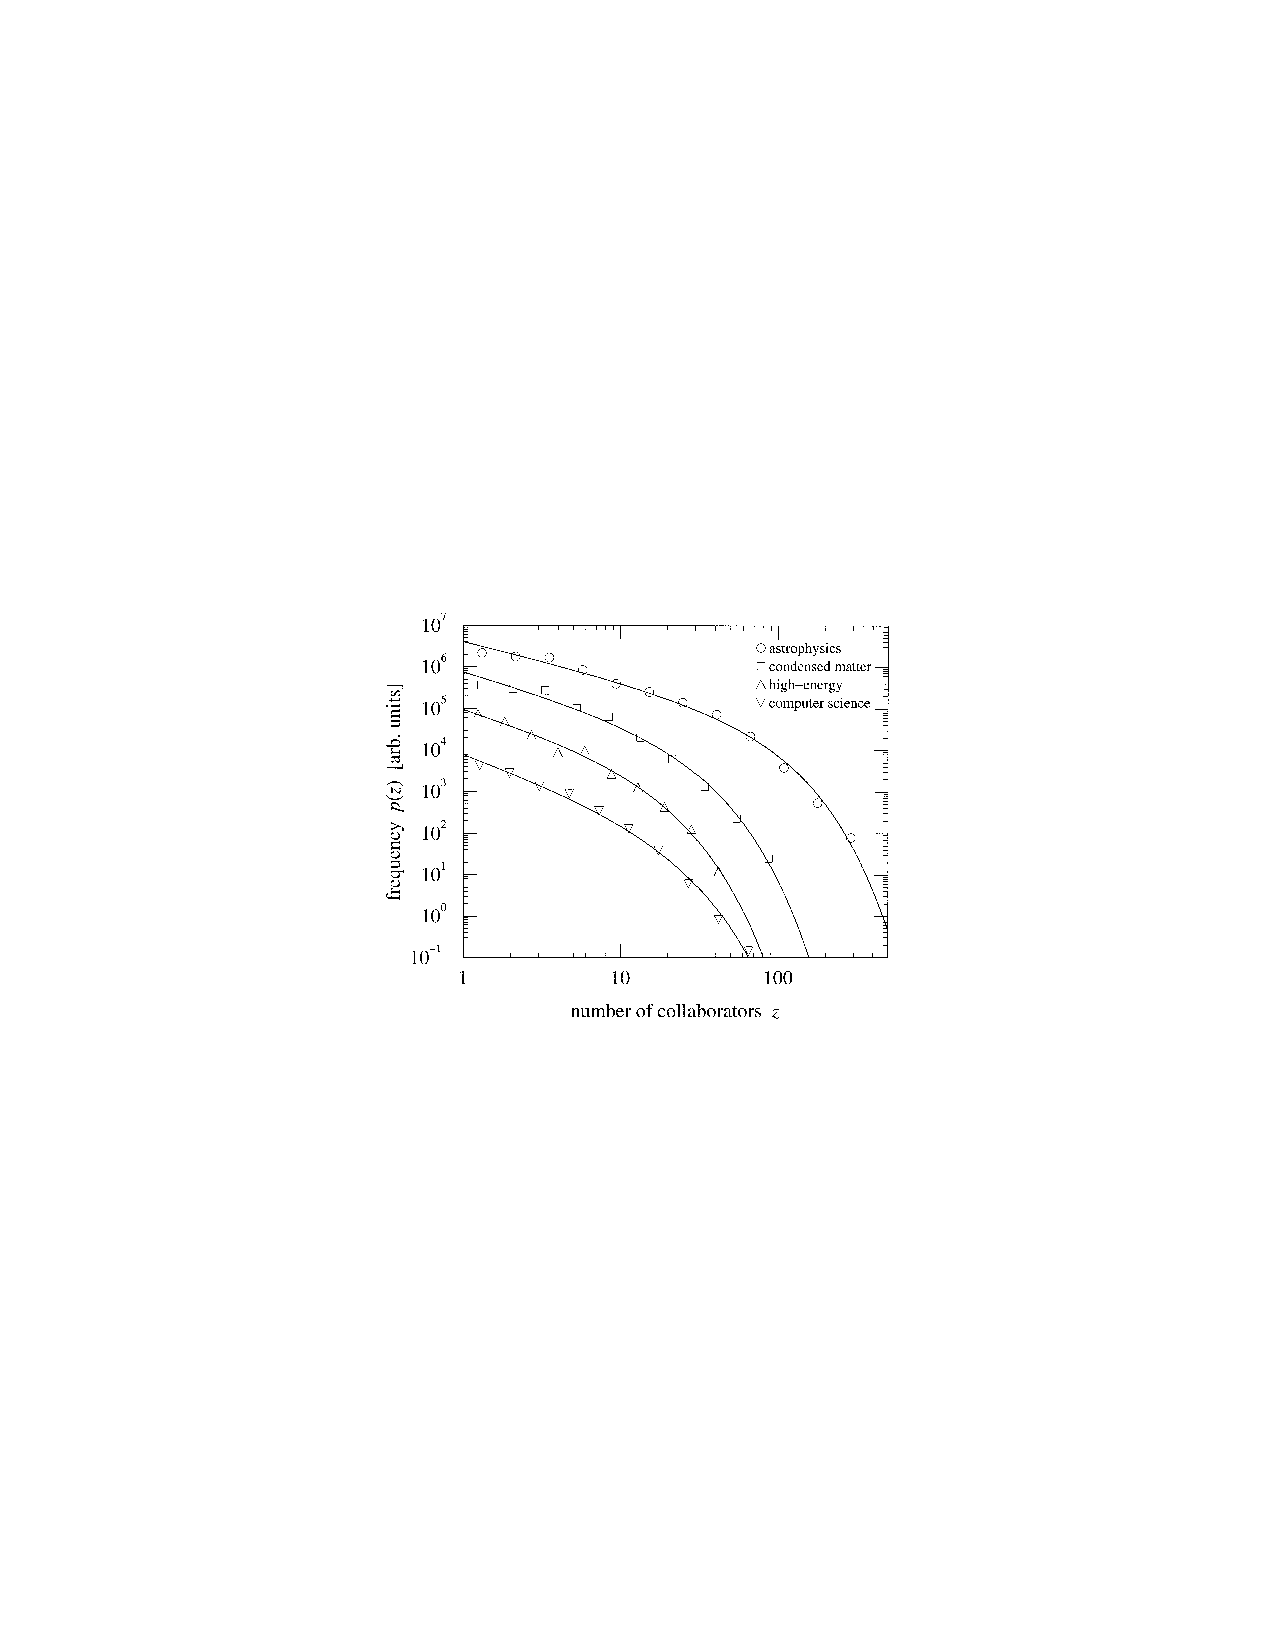
\includegraphics[scale=1]{coauthorship.pdf}
	\caption{In the coauthorship network of researchers, a vertex in the graph denotes a researcher, and two vertices are connected if the two researchers have published a paper together. This figure shows the degree distribution of vertices in the coauthorship network of researchers in astrophysics, condensed matter physics, high-energy physics, and computer science. Dots denote observed data, curves are fitted using \hyperref[eqn:truncated_power_law]{equation~\ref{eqn:truncated_power_law}}. In all four cases, the fit yields Pearson's $r^2$ higher than 0.99.}
	\label{fig:coauthorship}
\end{figure}

The freedom of distribution allows a new way to look at the process of generating random graphs. With $N$ vertices, we can assign each of them $z$ ``stubs'', or ends of edges, where $z$ is decided by arbitrary probabilistic distribution function $p(z).$ Then we randomly choose stubs in pair and connect them. If the total number of stubs happens to be odd, we can just start all over again.

\section{From Percolation to Giant Component}

The theory of percolation is introduced with fractals in Chapter 8. Because in social networks, it is natural to assume the existence of isolated communities, so instead of percolation, we study the dynamics of giant component. According to \cite{wiki_giant_component}, a giant component is a connected subgraph whose size is a constant fraction of the entire graph, i.e.\ $s\sim O(n).$

In an \ER random graph, where we denote the probability of each possible edge being chosen by $k/n,$ there is a point of phase transition at $k=1.$ For $k<1,$ the graph generally contains many relatively small communities, and they tend to have size $s\sim O(log(n)).$ For $k>1,$ on the other hand, the graph is generally dominated by a giant component, while all smaller communities still have size $s\sim O(log(n)).$

However, note that such estimation is based on the unrealistic vertex degree distribution of the \ER model. For an arbitrary distribution of vertex degree, a different approach is required. According to \cite{newman2002random}, using generating functions to (asymptotically) approximate \hyperref[eqn:truncated_power_law]{equation~\ref{eqn:truncated_power_law}}, a curve of phase transition is analytically found on the $\tau-z_c$ plane. The generating function method also allows the exact solution of other properties such as the average path length between vertices, and has been widely applied to different vertex degree distributions. The detail of mathematical derivations is beyond the scope of this case study, but the result is shown in \hyperref[fig:giant_component]{figure~\ref{fig:giant_component}}.

\begin{figure}[htbp]
	\centering
	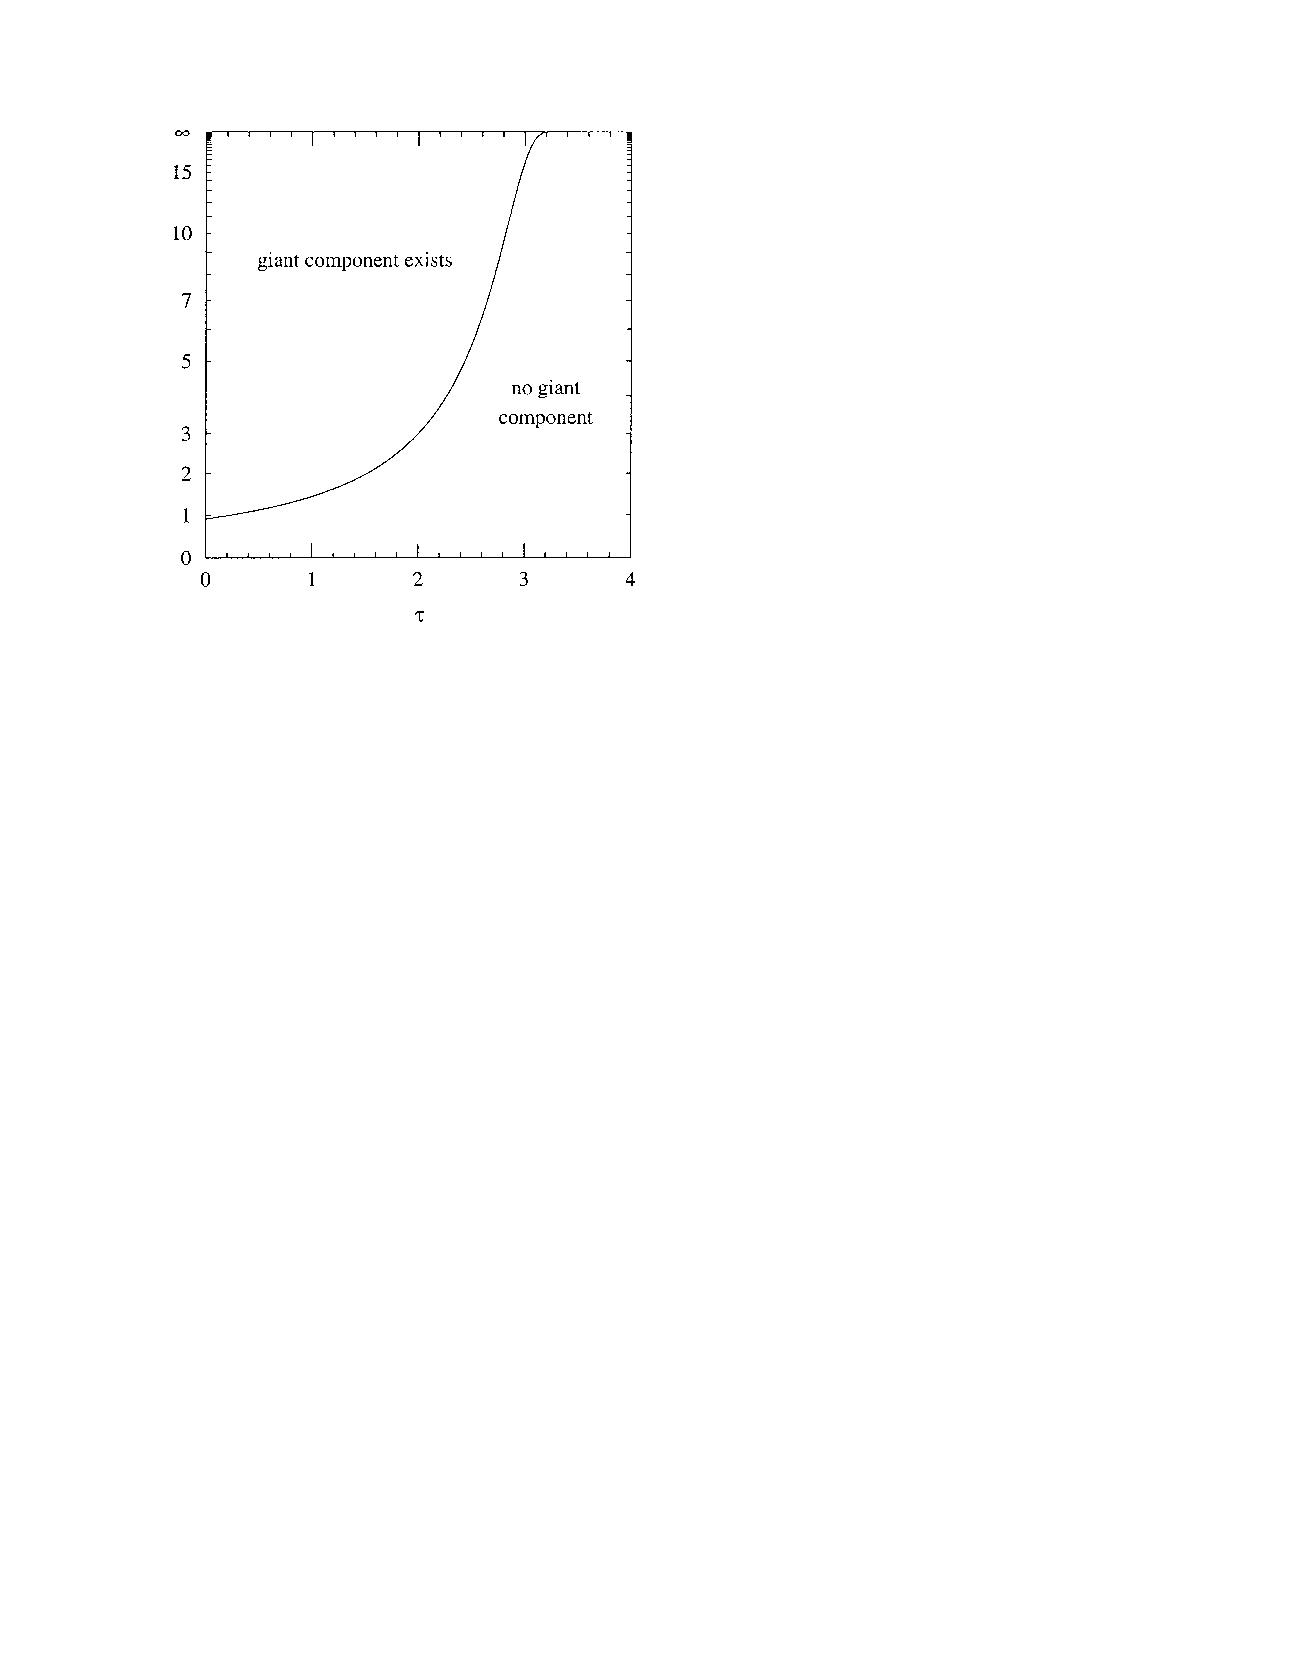
\includegraphics[scale=1]{giant_component.pdf}
	\caption{Phase diagram on the $\tau-z_c$ plane of random graph with \hyperref[eqn:truncated_power_law]{equation~\ref{eqn:truncated_power_law}} as vertex degree distribution. The solid curve marks the boundary between the region in which a giant component exists and one that it does not. Most observed social networks have giant components.}
	\label{fig:giant_component}
\end{figure}

\section{Analysis of the Facebook Social Graph}

In 2011, Facebook published an analysis \cite{ugander2011anatomy} on its social graph. Due to the size of Facebook user group (721 million at the time of analysis), this analysis provided invaluable resource to the research of complex system, especially the design of algorithms that work on such graphs. A few highlights of the analysis are described below, and illustrated in \hyperref[fig:facebook]{figure~\ref{fig:facebook}}:

%\topsep: space between first item and preceding paragraph; \partopsep: extra space added to \topsep when environment starts a new paragraph; \itemsep: space between successive items.
\begin{enumerate}[topsep=0pt,itemsep=-1ex,partopsep=1ex,parsep=1ex]
\item The top-left subgraph shows the degree distribution of users. The sharp drop at 5000 is due to the upper limit of the number of friends one can have. Although both shapes (the global user graph and the subgraph of 149 million U.S.\ users, respectively) are visually similar to \hyperref[fig:coauthorship]{figure~\ref{fig:coauthorship}}, no statistical tests are done in the report.\footnote{It is noteworthy here that with such a big number of users, traditional statistical methods may be unreliable.} The median friend count of global users is 99.
\item The top-right subgraph shows the cumulative distribution of distance between users. The theory of six degree separation is confirmed (again) in this test. Also note the steep slope between 3 and 4. The average distance between a pair of global users is 4.7, while the average distance between a pair of U.S.\ users is 4.3. Overall, more than 99.9\% of global users belong to a giant component.
\item The bottom-left subgraph shows the clustering coefficient, as introduced in the Watts-Strogatz model (Chapter 4). According to this chart, the Facebook social graph is moderately dense. For example, 14\% of all possible friend pairs around a user with 100 friends (almost median) are themselves friends. The sharp drop near 5000 degrees suggests that super users are adding friends indiscriminately.
\item The bottom-right subgraph shows the degeneracy. Formally, the degeneracy of a graph $G$ is defined as the largest $k$ such that $G$ has a non-empty subgraph $H$ in which all vertices have degree greater than or equal to $k.$ Intuitively, degeneracy measures the size of the largest ``clique'' among the friends of a user. According to this chart, there exist surprisingly large tight communities within one's friend circle. This idea shall be revisited in \hyperref[sec:affiliation]{section~\ref{sec:affiliation}}.
\end{enumerate}

As a final word of this section, the Facebook report does not include any temporal analysis of its social graph. For interested readers, a brief analysis on the temporal evolution of the Flickr and Yahoo! 360 social network can be found in \cite{kumar2010structure}.

\begin{figure}[htbp]
	\centering
	\begin{subfigure}
		\centering
		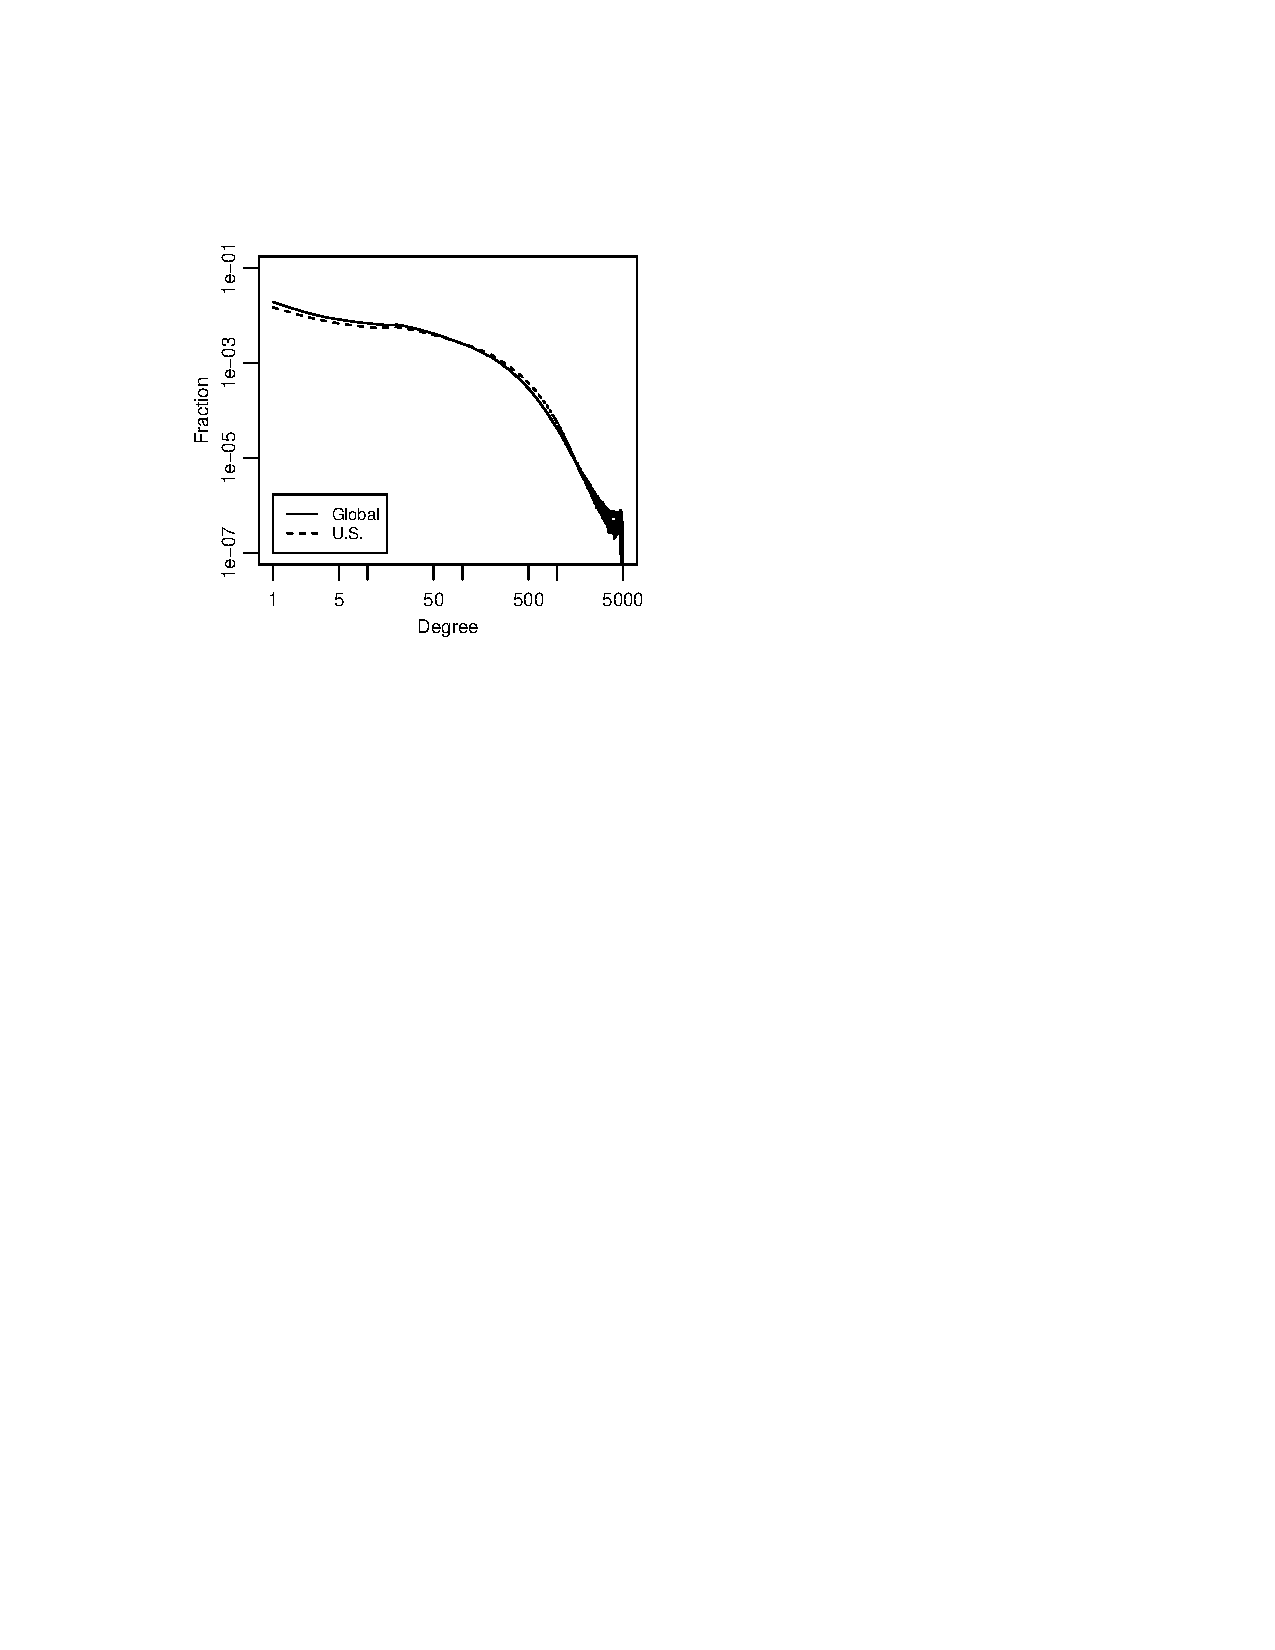
\includegraphics[scale=0.95]{fb_degree.pdf}
	\end{subfigure}
	\begin{subfigure}
		\centering
		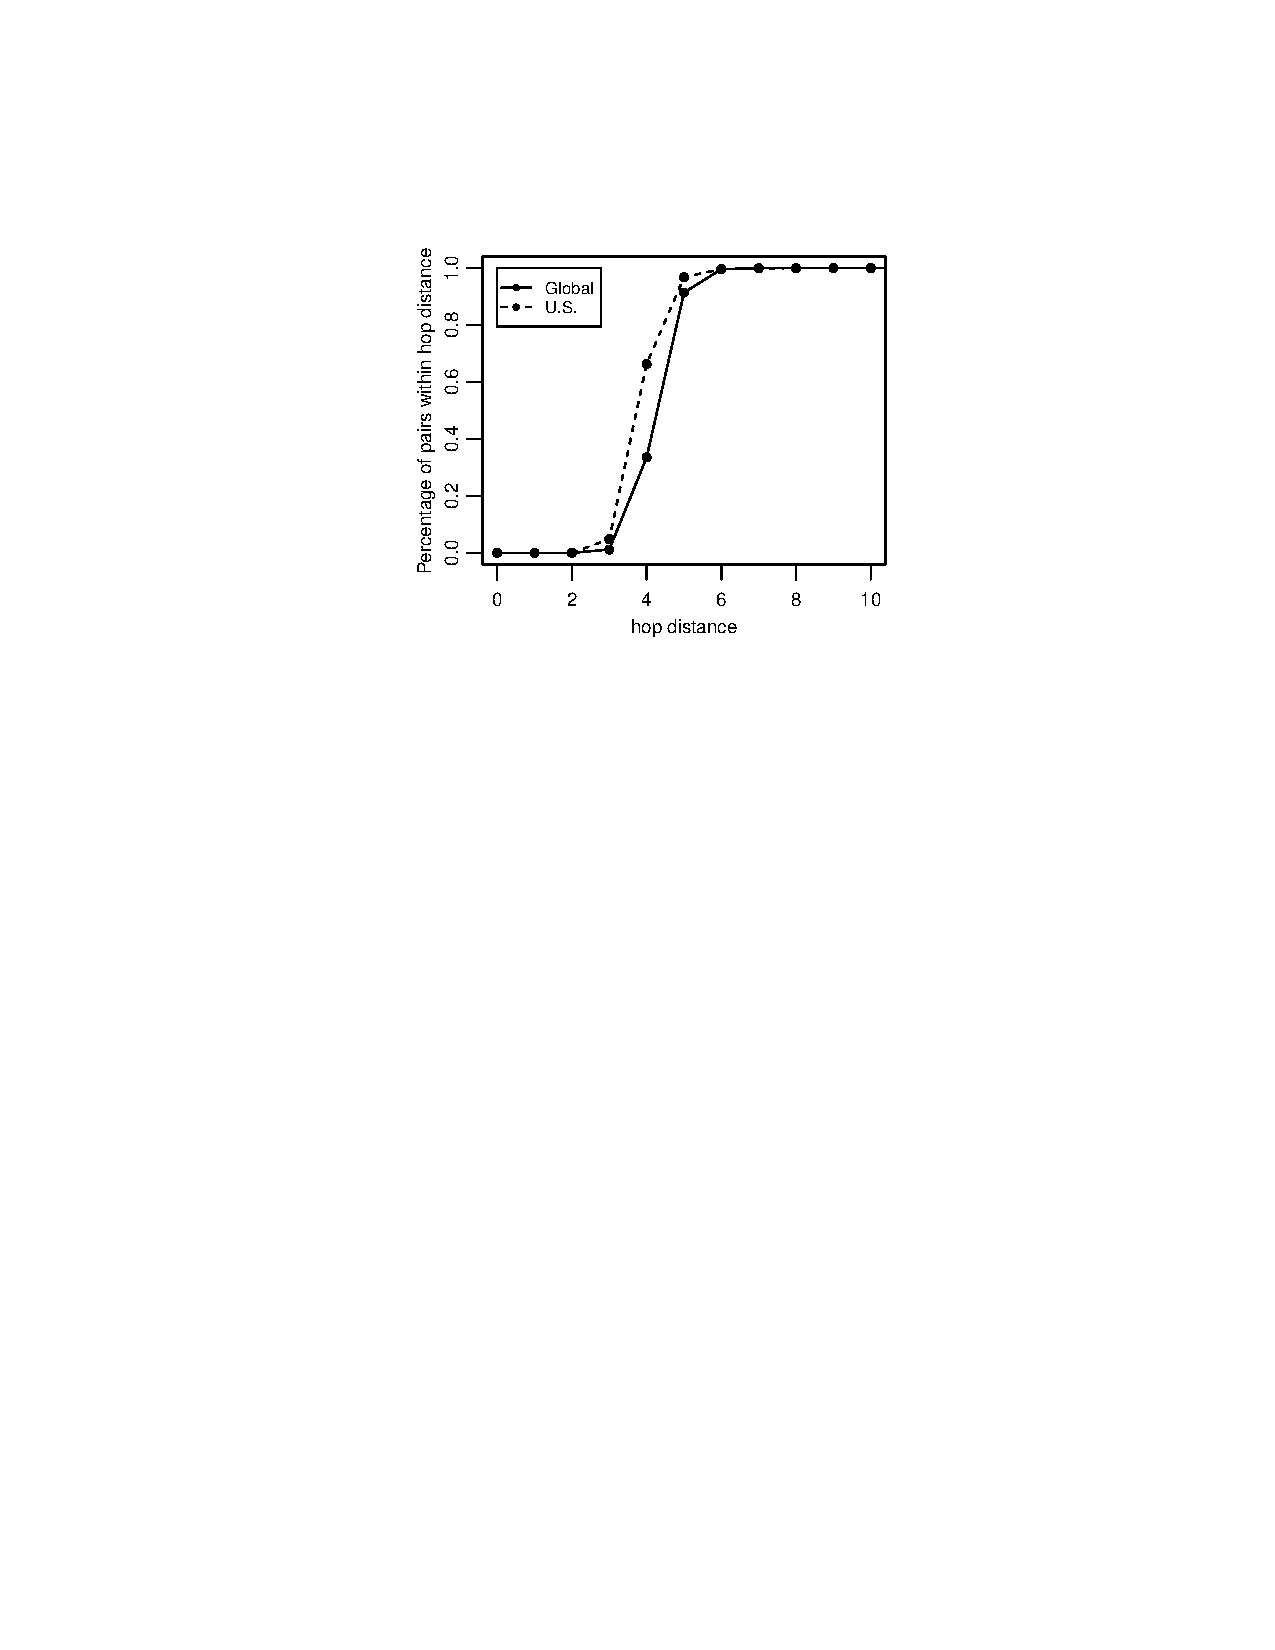
\includegraphics[scale=0.95]{fb_distance.pdf}
	\end{subfigure}
	\begin{subfigure}
		\centering
		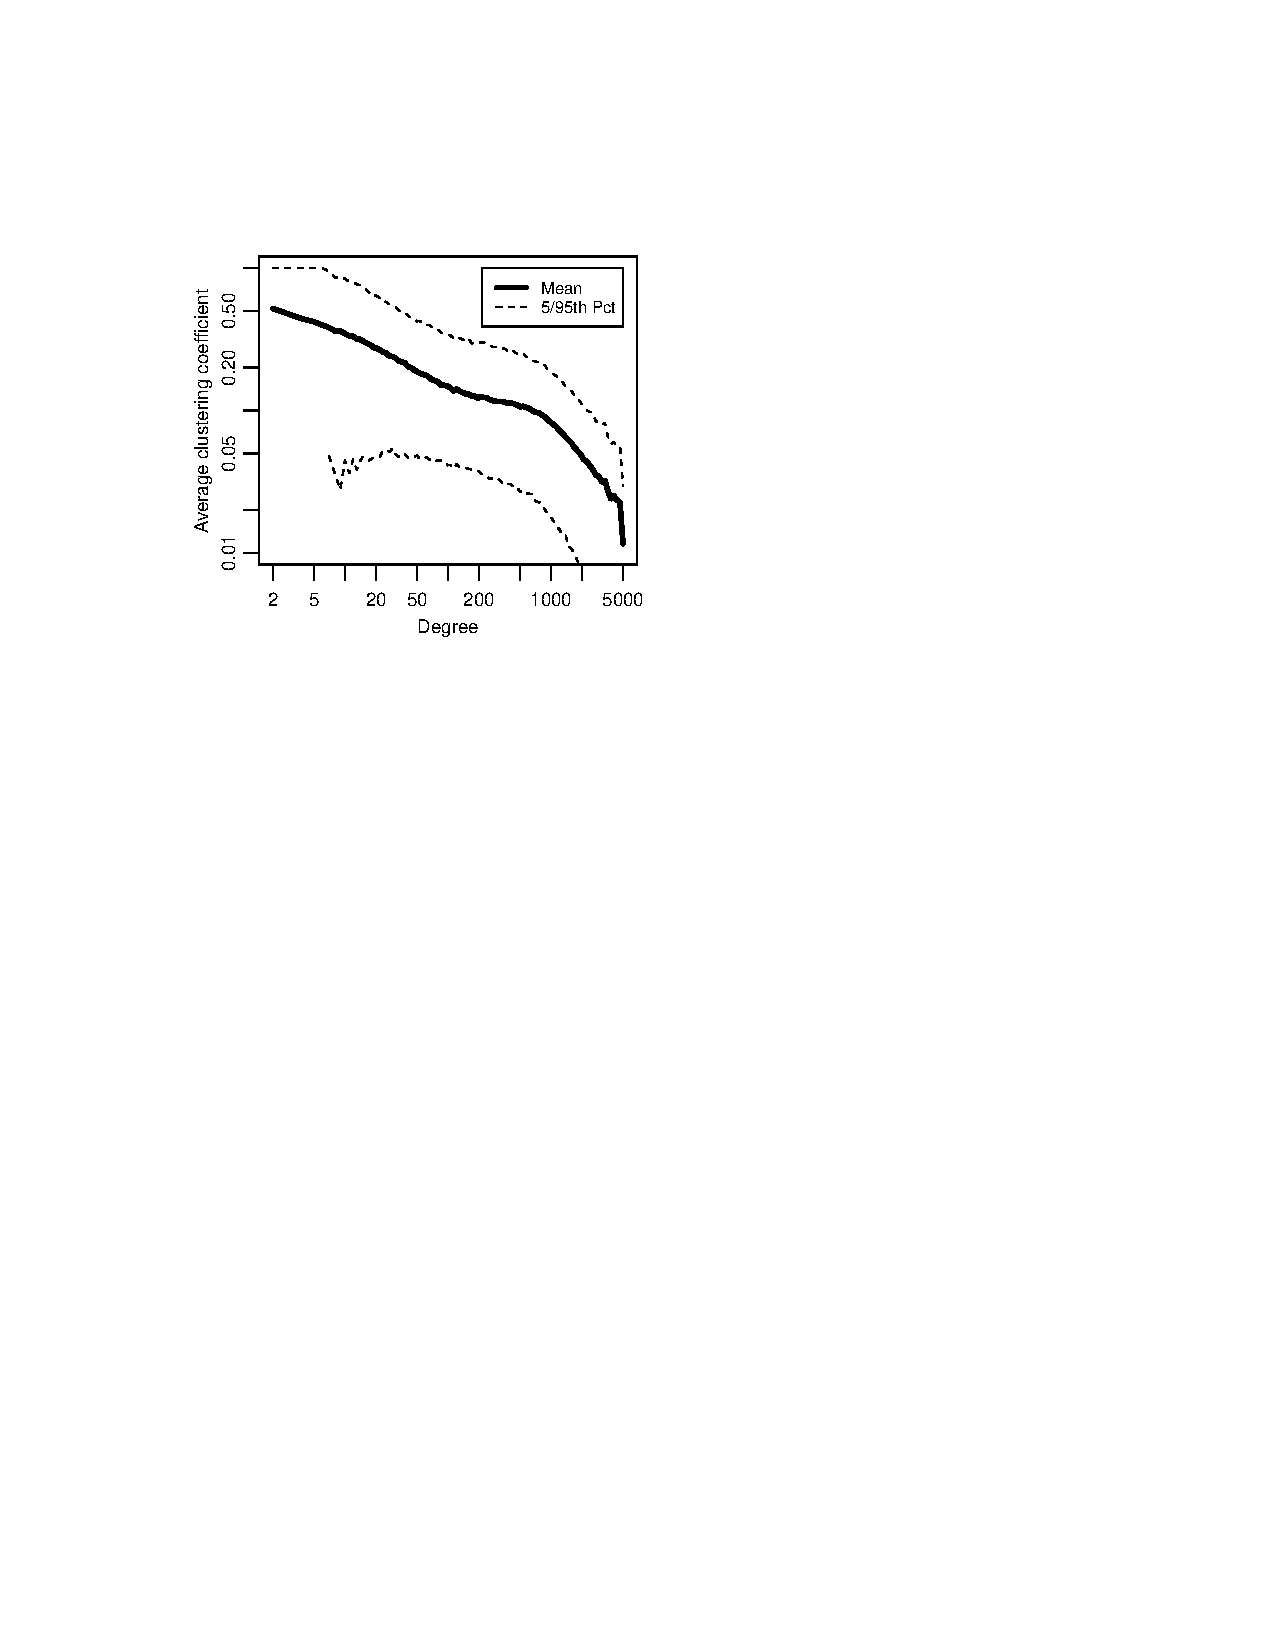
\includegraphics[scale=0.95]{fb_cluster.pdf}
	\end{subfigure}
	\begin{subfigure}
		\centering
		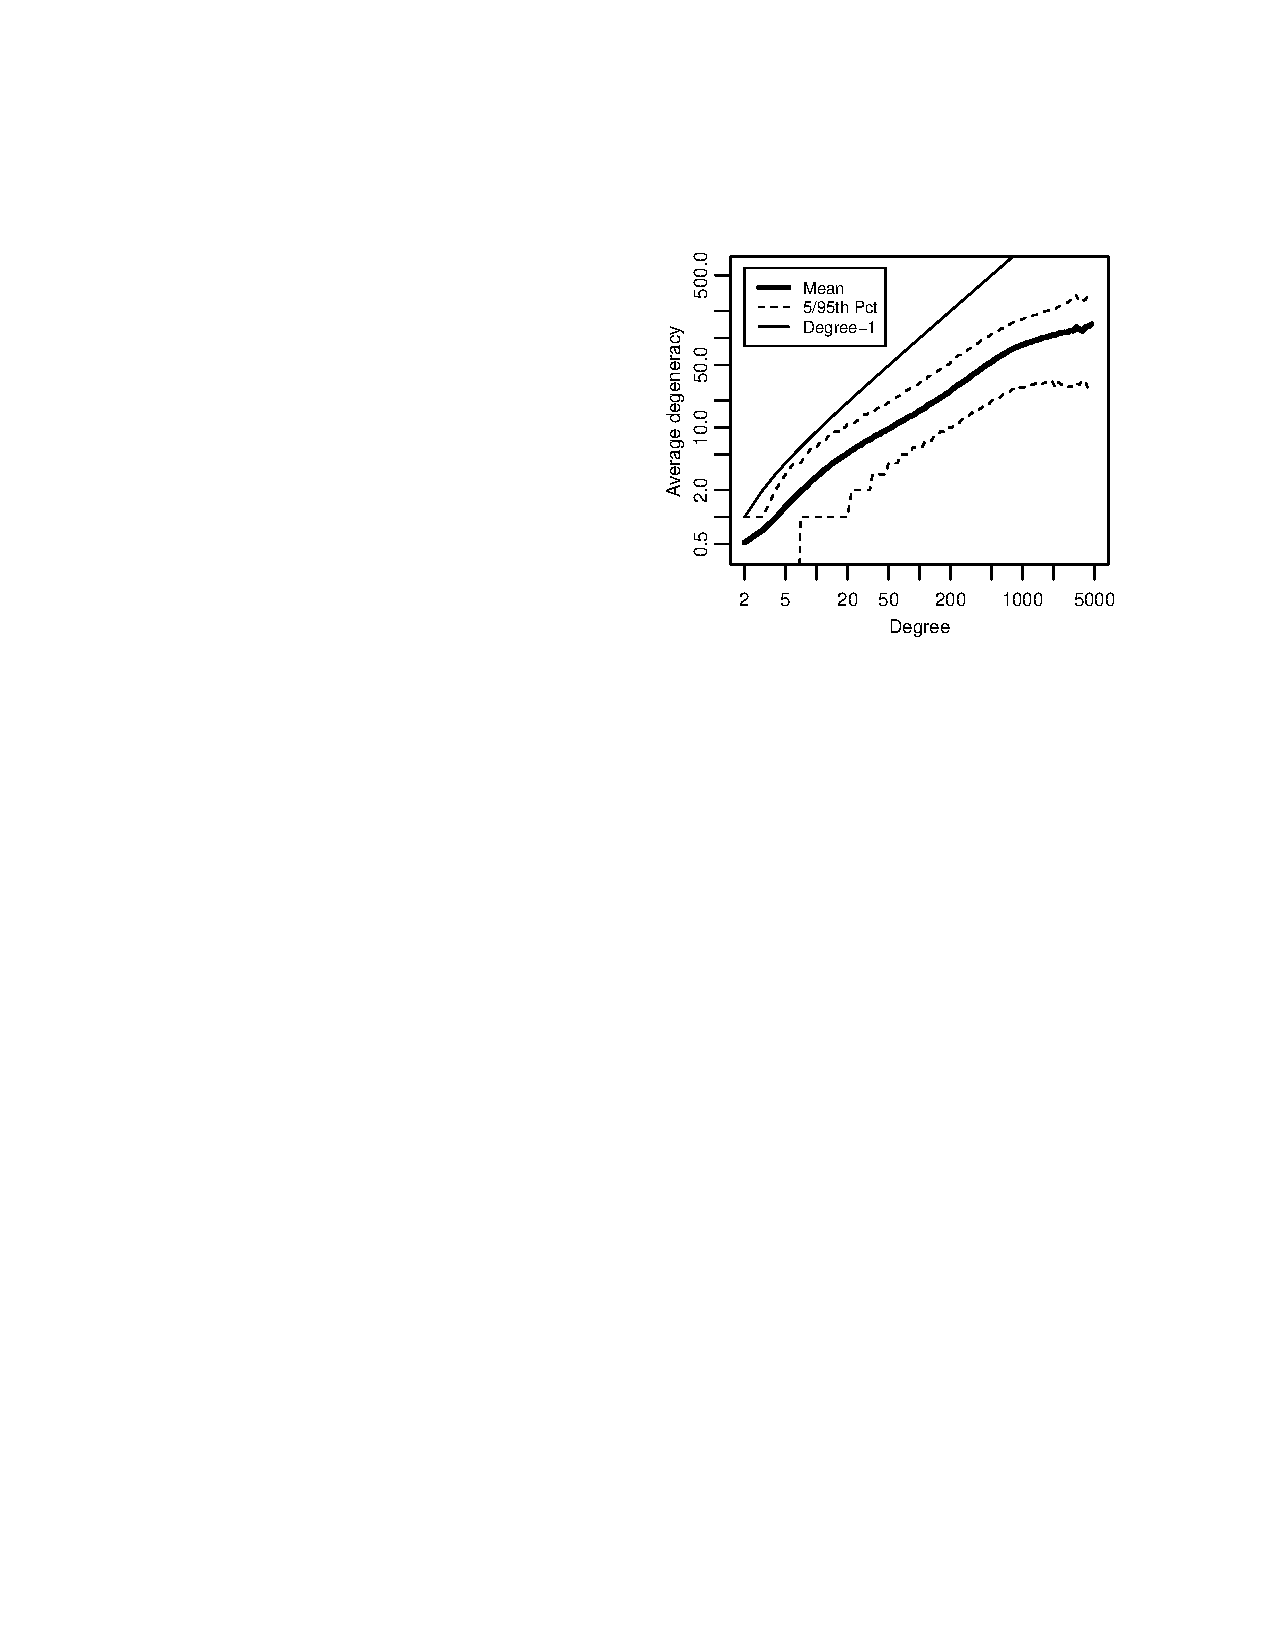
\includegraphics[scale=0.95]{fb_degeneracy.pdf}
	\end{subfigure}
	\caption{Analysis of the Facebook social graph.}
	\label{fig:facebook}
\end{figure}

\section{Modelling the Affiliation Network}
\label{sec:affiliation}

It is common in social networks that people in a ``group'' all know each other. For example, researchers who collaborate on a paper \cite{newman2001structure}, actors who cast in a movie, Facebook users who know at the workplace. Such structure can be modeled as an affiliation network, as shown in \hyperref[fig:affiliation]{figure~\ref{fig:affiliation}}:

\begin{figure}[htbp]
	\centering
	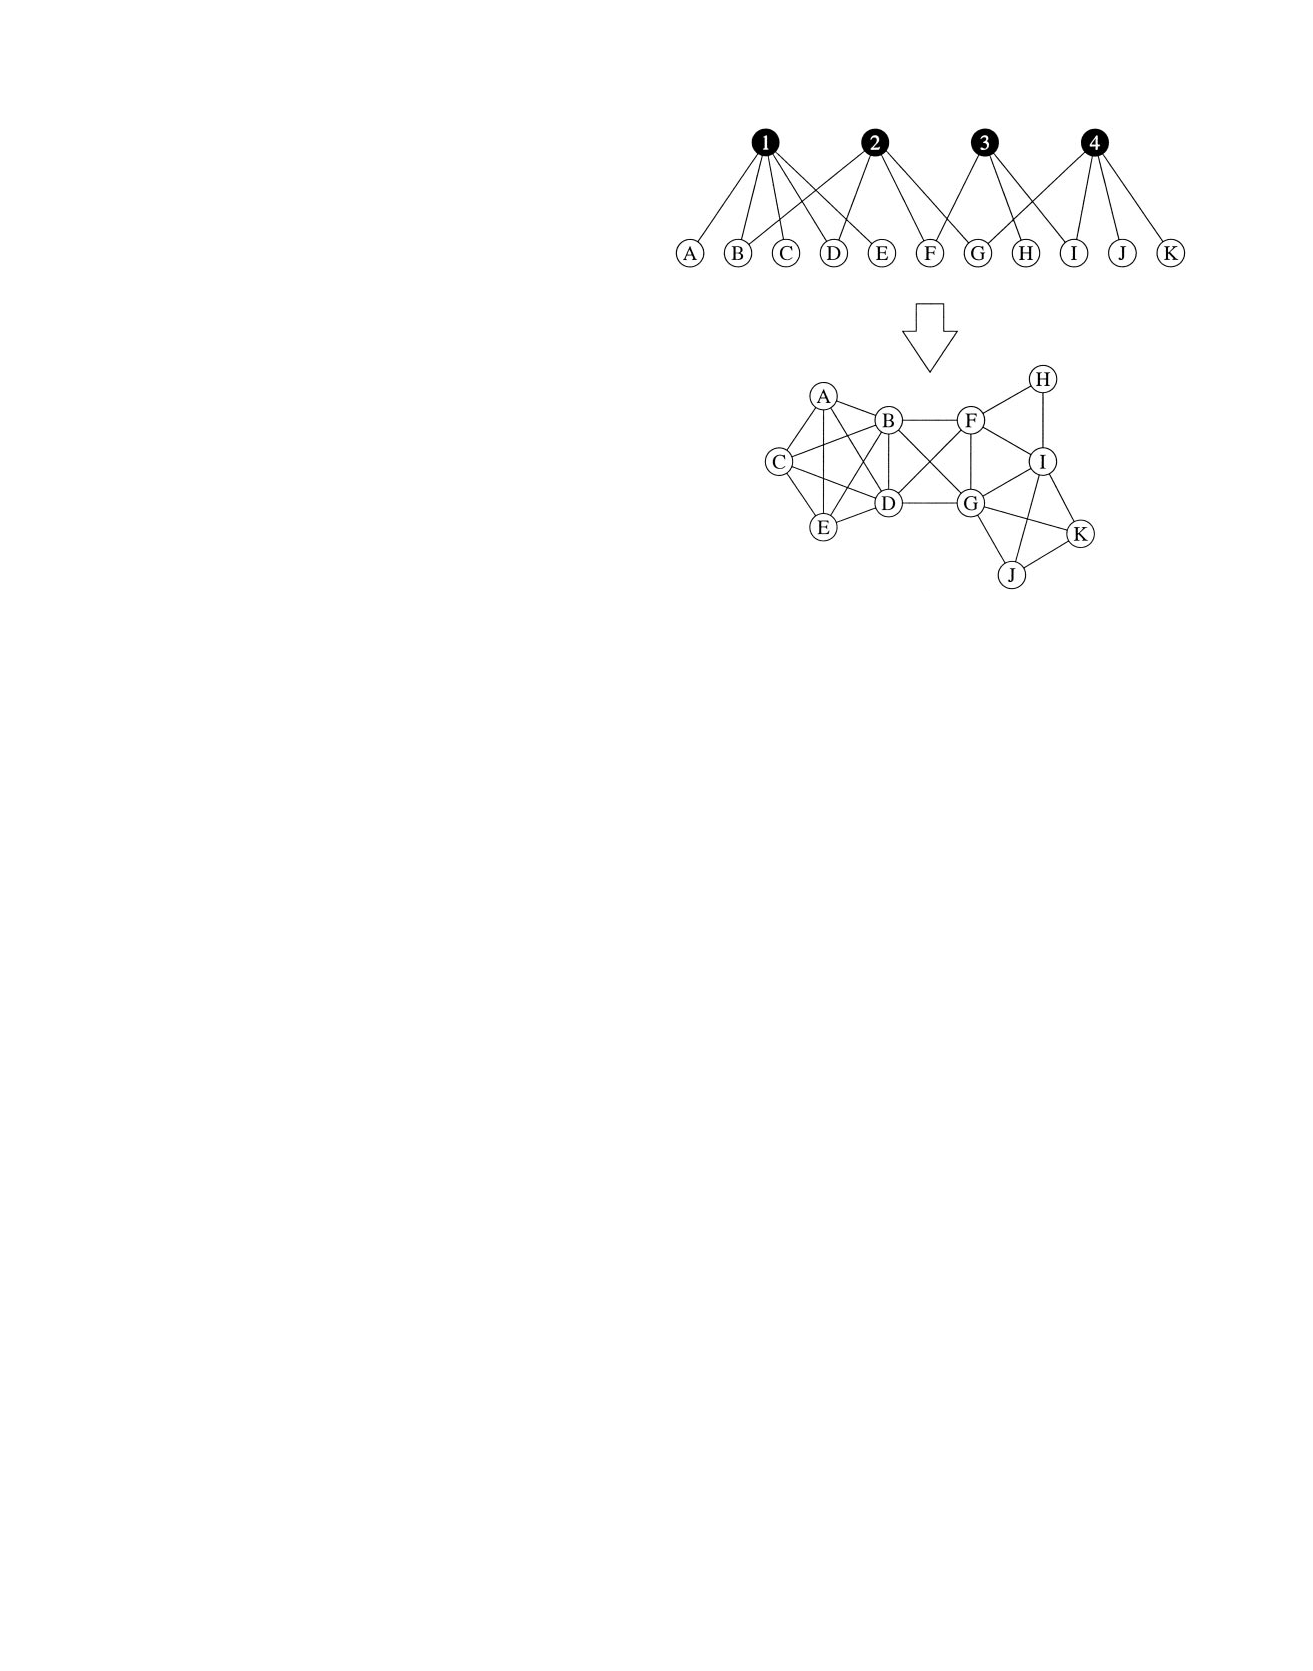
\includegraphics[scale=1]{affiliation.pdf}
	\caption{An affiliation network can be generated from a bipartite graph, but not the other way. In the bipartite graph, white vertices denote agents, while black vertices denote projects in which agents collaborate. In the lower graph, white vertices still denote agents, and two vertices are connected if they are connected to the same black vertex in the bipartite graph.}
	\label{fig:affiliation}
\end{figure}

Because an affiliation network is effectively a union of many small complete graphs, they tend to have relatively high clustering coefficient and degeneracy. In this section, we propose a social model that approaches the structure of the scientific coauthorship network of arXiv papers on theoretical high energy physics \cite{stanford_network_dataset}, a social network with $9,877$ vertices (authors) and $51,971$ edges (collaborations). The dataset does not contain the associated bipartite graph.

The algorithm generates the affiliation network by creating the bipartite graph in two passes. In the first pass, as a start point, each of $9,877$ authors is indiscriminately assigned to a project group, whose size follows the right hand side of normal distribution $N(\mu=2, \sigma=2).$ This distribution is part of the modelling assumptions. Then the second pass runs in a loop, shown as follows:
\begin{enumerate}[topsep=0pt,itemsep=-1ex,partopsep=1ex,parsep=1ex]
\item The algorithm creates an empty project group with $m$ places, where $m$ follows the right hand side of $N(\mu=2, \sigma=2).$
\item As the first author of the project group, the algorithm selects an author on a roulette wheel with fitness function:
\[f(k)=c+p(k)-e^{p(k)/20}\]
where $c$ is a small constant, and $p(k)$ is the total number of collaboration of author $k$ so far. Note that $p(k)$ does not necessarily correspond to the degree of vertex $k$ in the affiliation network, since an edge between two authors do not tell how many times they have collaborated. Intuitively, $p(k)$ and $e^{p(k)/20}$ denote the experience and age of a researcher, respectively. The negative effect of age overruns experience at $p(k)\approx95.$
\item The rest of the project group are selected in a greedy manner. For each position left, the algorithm selects an author on a roulette wheel from the friend circle of selected authors with fitness function:
\[g(k)=c+p(k)-e^{p(k)/20}+100\cdot q(k)\]
where $q(k)$ is the total number of collaborations that author $k$ have had with any selected group members so far. In other words, the project group countinuously expands its range of selection for the next member. This process is designed to simulate the friend suggestion mechanism of online social network services, with which two users have a higher chance to become friends if they are not friends yet, but have many friends in common. When the friend circle of selected group is empty, or at a very small chance, the algorithm makes the selection from the set of all authors.
\item The algorithm terminates when the number of edges in the affiliation network have reached the predefined limit of $51,971.$
\end{enumerate}
The result analysis of the experiment is shown in the following figures:
\begin{figure}[htbp]
	\centering
	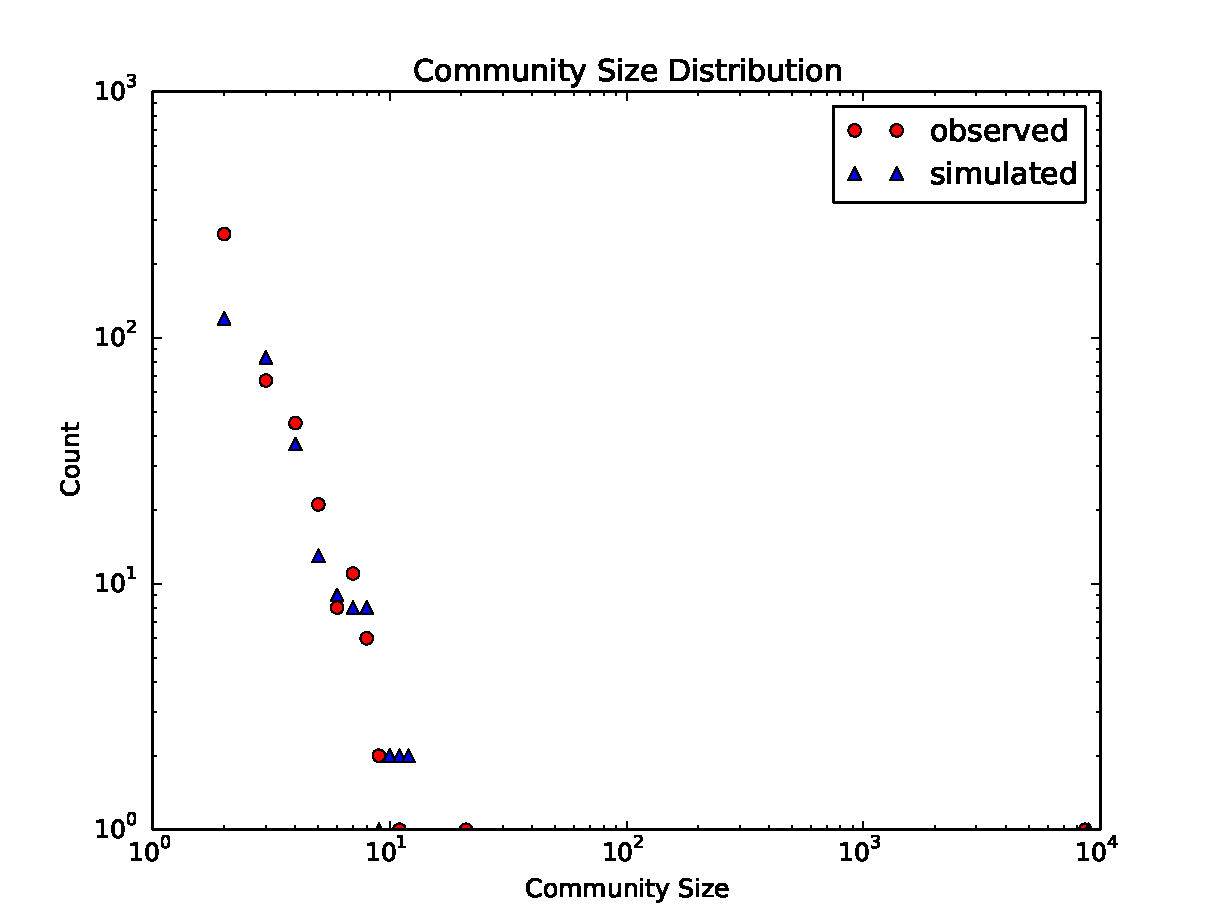
\includegraphics[scale=0.55]{exp_community_size_distro.pdf}
	\caption{Number of communities of different sizes on a log-log scale. A power law is clearly visible on the left side, whereas the giant component on the bottom-right corner contains the majority of authors.}
	\label{fig:exp_community_size_distro}
\end{figure}
\begin{figure}[htbp]
	\centering
	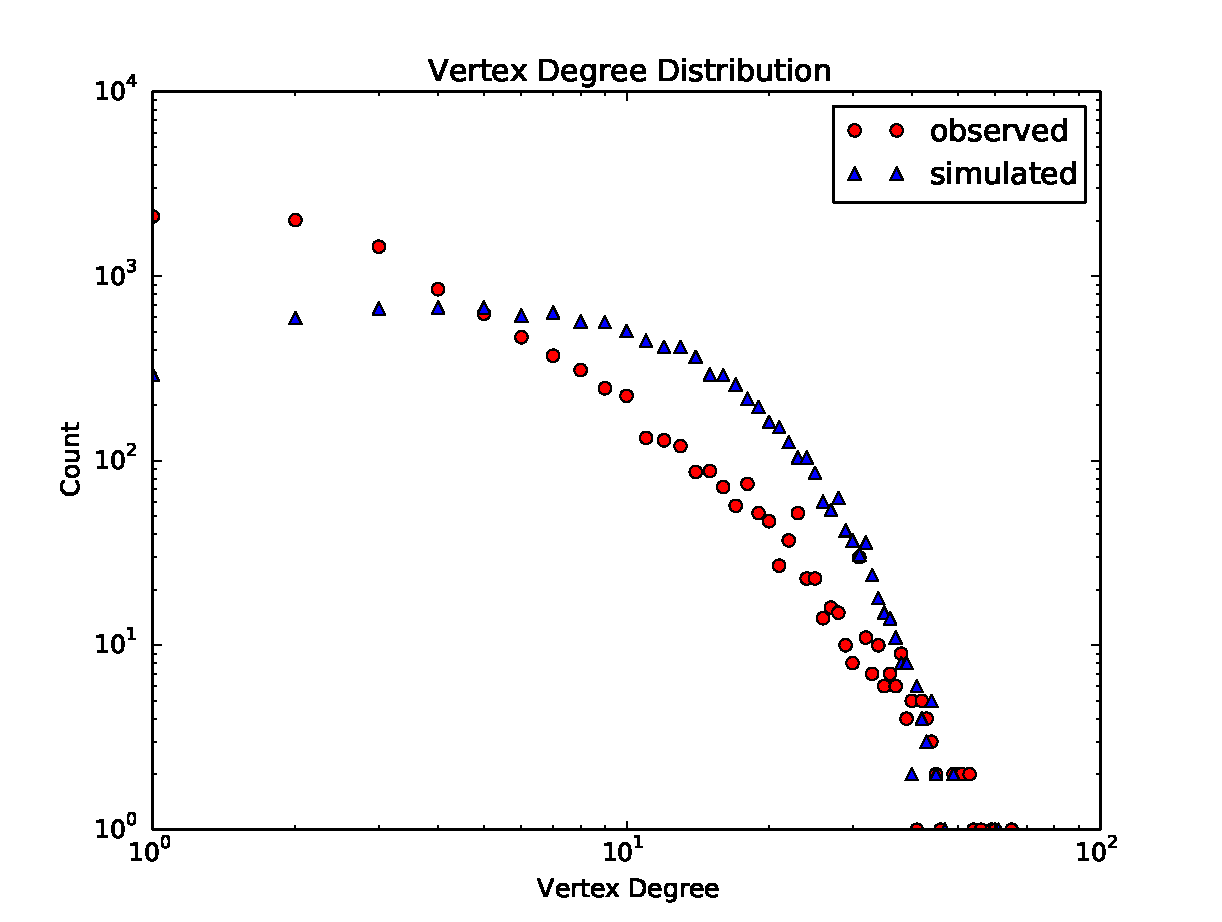
\includegraphics[scale=0.55]{exp_degree_distro.pdf}
	\caption{Number of vertices of different degrees on a log-log scale. While the observed data follows the power law, the simulated network seems to have a strong suppress effect on vertices with both very high degree and very low degree.}
	\label{fig:exp_degree_distro}
\end{figure}
\begin{figure}[htbp]
	\centering
	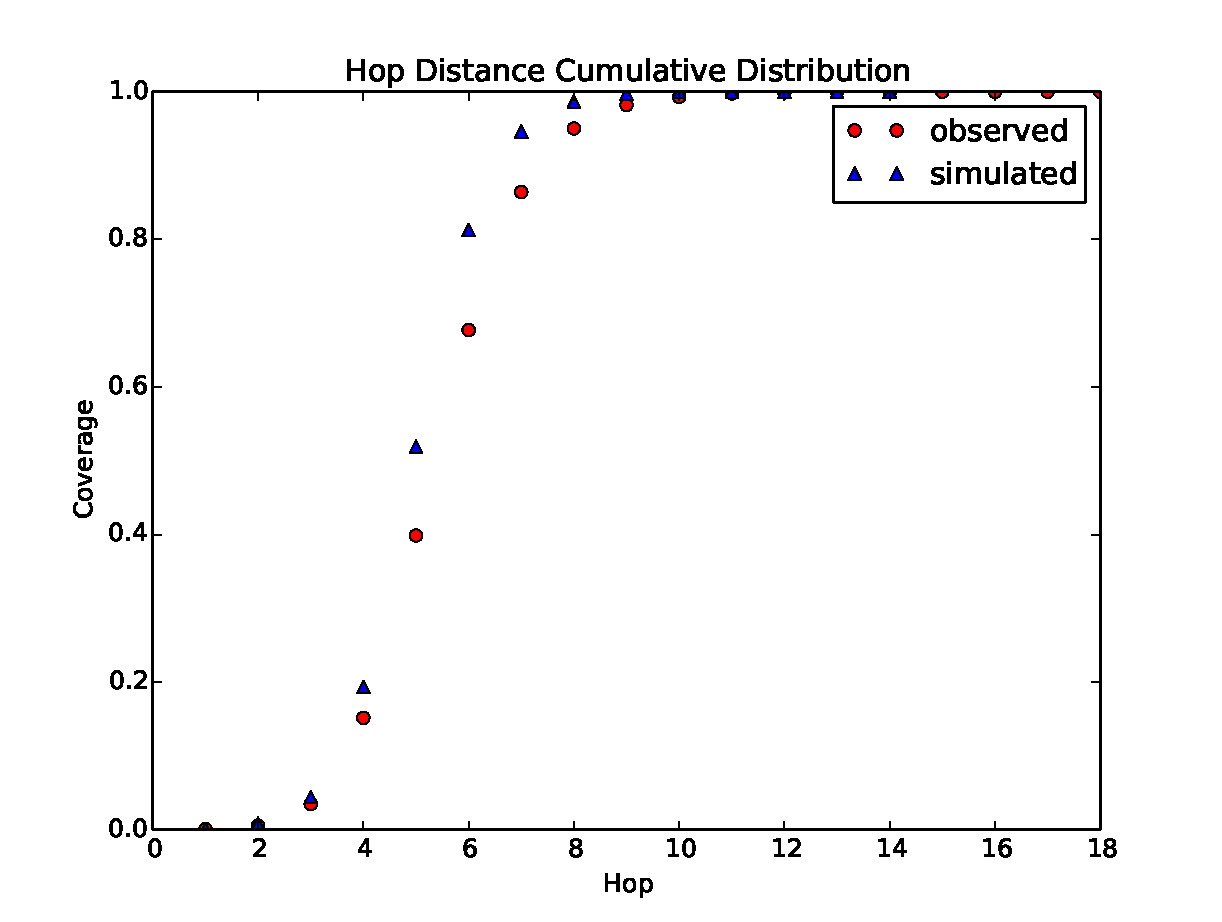
\includegraphics[scale=0.55]{exp_hop_distro.pdf}
	\caption{Cumulative distribution of hop distance. The majority of vertices can be reached in 8 hops in both networks, slightly longer than in the real world. This is a clear sign of local clustering of the theoretical high energy physics community.}
	\label{fig:exp_hop_distro}
\end{figure}
\begin{figure}[htbp]
	\centering
	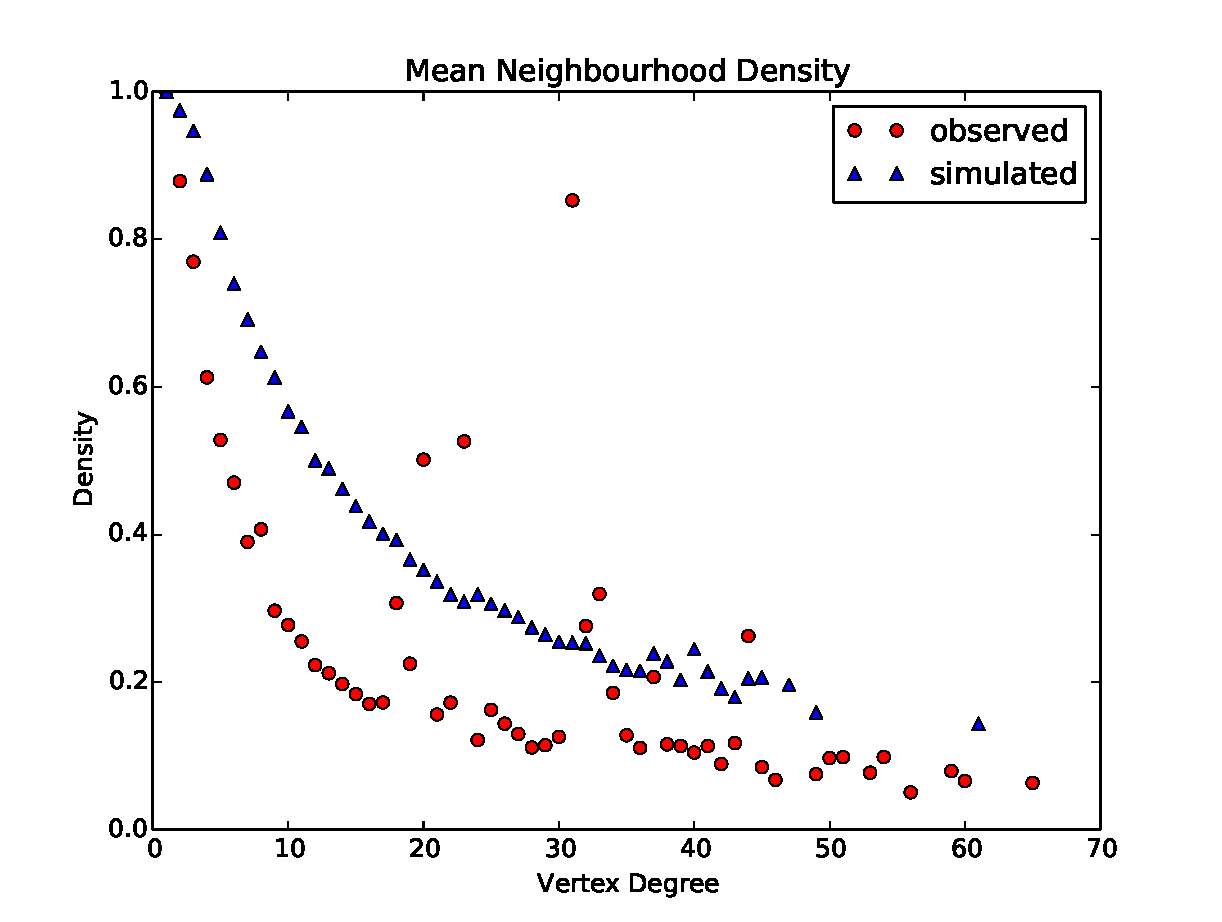
\includegraphics[scale=0.55]{exp_neighbourhood_densities.pdf}
	\caption{Average clustering coefficients of vertices of different degrees. The simulated network shows similar trend to the observed network, but tends to have slightly higher clustering coefficient.}
	\label{fig:exp_neighbourhood_densities}
\end{figure}
\begin{figure}[htbp]
	\centering
	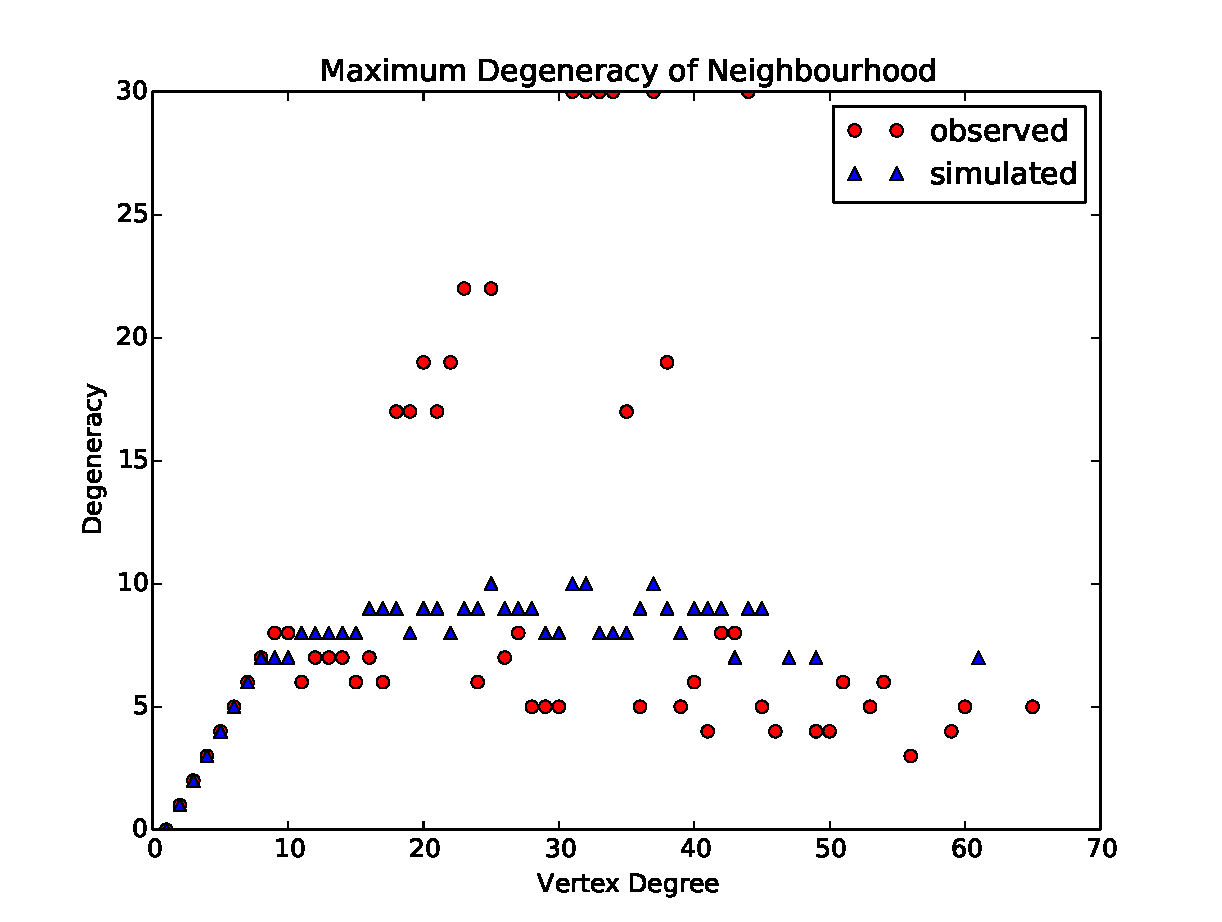
\includegraphics[scale=0.55]{exp_max_degeneracies.pdf}
	\caption{Maximum degeneracy of vertices of different degrees. Interestingly, in both networks, the maximum degeneracy plateaus at around 7 for vertices with 10 degrees or higher. However, in the observed network, there are a few vertices that keep growing linearly, and eventually reach a plateau at 30.}
	\label{fig:exp_max_degeneracies}
\end{figure}

\clearpage
\bibliographystyle{plain}
\bibliography{Report}

\end{document}
